\documentclass[12pt,a4paper]{report}

\usepackage[utf8]{inputenc}
\usepackage[T1]{fontenc}
\usepackage[indonesian]{babel}
\usepackage{mathptmx}
\usepackage[a4paper,top=2.5cm,bottom=2.5cm,left=3cm,right=2.5cm]{geometry}
\usepackage{setspace}
\usepackage{graphicx}
\usepackage{float}
\usepackage{array}
\usepackage{longtable}
\usepackage{multirow}
\usepackage[table]{xcolor}
\usepackage{amsmath,amssymb}
\usepackage{enumitem}
\usepackage{caption}
\usepackage{titlesec}
\usepackage{tocloft}
\usepackage{listings}
\usepackage[hidelinks]{hyperref}

\onehalfspacing
\emergencystretch=3em
\setlength{\parindent}{1.25cm}
\setlength{\parskip}{0pt}
\graphicspath{{img/}{../../output/}}

% ---------- gaya bab dan subbab (mengikuti laporan sebelumnya) ----------
\titleformat{\chapter}[display]{\centering\bfseries\large}{BAB \Roman{chapter}}{0pt}{\large\MakeUppercase}
\titlespacing*{\chapter}{0pt}{0pt}{24pt}
\titleformat{\section}{\bfseries\normalsize}{\thesection.}{1em}{}
\titleformat{\subsection}{\bfseries\normalsize}{\thesubsection.}{1em}{}
\renewcommand{\thesection}{\arabic{chapter}.\arabic{section}}

\titleformat{name=\chapter,numberless}{\centering\bfseries\large}{}{0pt}{\MakeUppercase}
\titlespacing*{name=\chapter,numberless}{0pt}{0pt}{24pt}
\renewcommand{\thechapter}{\Roman{chapter}}
\renewcommand{\thetable}{\arabic{chapter}.\arabic{table}}
\renewcommand{\thefigure}{\arabic{chapter}.\arabic{figure}}
\addto\captionsindonesian{\renewcommand{\contentsname}{DAFTAR ISI}%
  \renewcommand{\bibname}{DAFTAR PUSTAKA}}
\renewcommand{\cfttoctitlefont}{\hfill\bfseries\large}
\renewcommand{\cftaftertoctitle}{\hspace*{\fill}}
\setlength{\cftbeforetoctitleskip}{0pt}
\renewcommand{\cftchapfont}{\bfseries}
\renewcommand{\cftchappagefont}{\bfseries}
\renewcommand{\cftchappresnum}{BAB }
\setlength{\cftchapnumwidth}{5em}
\renewcommand{\cftchapleader}{\cftdotfill{\cftdotsep}}

\captionsetup{labelsep=space,font=small,labelfont=bf,justification=centering}
\captionsetup[table]{position=above}
\renewcommand{\tablename}{Tabel}
\renewcommand{\figurename}{Gambar}

\definecolor{hdr}{gray}{0.94}
\newcommand{\hd}[1]{\cellcolor{hdr}\textbf{#1}}
\newcolumntype{L}[1]{>{\raggedright\arraybackslash}p{#1}}
\newcolumntype{C}[1]{>{\centering\arraybackslash}p{#1}}
\renewcommand{\arraystretch}{1.35}

\lstset{basicstyle=\ttfamily\footnotesize,frame=single,breaklines=true,
        columns=fullflexible,keepspaces=true,showstringspaces=false}

\newcommand{\code}[1]{\texttt{\small #1}}

\begin{document}

% =====================================================================
%                              SAMPUL
% =====================================================================
\begin{titlepage}
\centering
\vspace*{1cm}
{\fontsize{20}{28}\selectfont\bfseries Laporan Tugas Besar 1\par}
\vspace{0.4cm}
{\fontsize{20}{28}\selectfont\bfseries IF3170 - Inteligensi Artifisial\par}
\vspace{1.2cm}
Dipersiapkan oleh\par
K01 - WeDaBest\par
\vspace{1.5cm}

\includegraphics[width=0.48\textwidth]{logo_itb.png}\par
\vspace{2cm}
\begin{tabular}{l@{\hspace{2.5cm}}l}
Muhammad Nur Majiid    & 13524028 \\[6pt]
Stefani Angeline Oroh  & 13524064 \\[6pt]
Angelina Andra Alanna  & 13524079 \\
\end{tabular}
\vfill
\end{titlepage}

\pagenumbering{arabic}
\setcounter{page}{2}
\tableofcontents

% =====================================================================
\chapter{DESKRIPSI PERSOALAN}
% =====================================================================

\section{Latar Belakang}
Mejiro Express adalah usaha logistik darat skala kecil milik keluarga Mejiro yang sedang
berada pada tahap uji coba. Pada tahap ini hanya tersedia satu (atau beberapa) truk dengan peti
kemas berukuran terbatas, sedangkan jumlah paket yang menunggu dikirim biasanya lebih banyak
daripada yang bisa diangkut. Penyusunan muatan secara manual memakan waktu dan sering kali
tidak optimal, sehingga dibutuhkan program yang dapat menentukan sendiri paket mana yang
dimuat, di posisi mana, dan dengan orientasi apa.

Secara formal, persoalan ini merupakan gabungan \textit{three-dimensional bin packing problem}
dan \textit{knapsack problem}. Selain mencari susunan geometris yang sah, program juga harus
memilih subset paket karena tidak semua paket muat sekaligus. Ruang pencariannya sangat besar,
sehingga pendekatan yang dipakai adalah \textit{local search}.

\section{Komponen Persoalan}
Persoalan melibatkan dua entitas, yaitu \textit{Package} (paket) dan \textit{Truck} (truk).
Atribut kedua entitas menjadi dasar representasi state, pengecekan constraint, dan perhitungan
nilai solusi. Ringkasannya ditunjukkan pada Tabel~\ref{tab:komponen}.

\begin{table}[H]
\centering
\caption{Entitas dan atribut persoalan}\label{tab:komponen}
\small
\begin{tabular}{|L{1.8cm}|L{2.4cm}|L{2.6cm}|L{6cm}|}
\hline
\hd{Entitas} & \hd{Atribut} & \hd{Contoh} & \hd{Keterangan} \\ \hline
\multirow{7}{*}{Package}
 & id & ``P4'' & Penanda unik paket \\ \cline{2-4}
 & Dimensions & \{w:6, l:3, h:2\} & Lebar, panjang, dan tinggi paket \\ \cline{2-4}
 & Orientation & \{w:y, l:x, h:z\} & Pemetaan sisi paket ke sumbu; ada enam kemungkinan \\ \cline{2-4}
 & Value & 70 & Nilai paket \\ \cline{2-4}
 & Weight & 40 & Berat paket \\ \cline{2-4}
 & IsFragile & True & Paket mudah pecah \\ \cline{2-4}
 & ETA & 2 & Sisa hari sampai paket harus tiba \\ \hline
\multirow{2}{*}{Truck}
 & Dimensions & \{w:6, l:6, h:4\} & Ukuran ruang peti kemas \\ \cline{2-4}
 & MaxCapacity & 100 & Batas total berat muatan \\ \hline
\end{tabular}
\end{table}

\section{Tujuan}
Tujuan persoalan adalah memaksimalkan jumlah \textit{value} paket yang berada di dalam peti kemas.
Paket yang ditinggalkan di luar truk tidak menyumbang nilai apa pun pada \textit{objective function}.

\section{Batasan (\textit{Constraint})}
Suatu susunan dinyatakan valid apabila seluruh syarat berikut terpenuhi:
\begin{enumerate}[leftmargin=1.5cm]
  \item Paket tidak menembus dinding: setiap paket harus sepenuhnya di dalam atau sepenuhnya
        di luar peti kemas.
  \item Paket tidak saling beririsan (\textit{overlap}) di dalam ruang yang sama.
  \item Paket tidak melayang: minimal satu titik alas paket ditopang oleh lantai atau atap paket lain.
  \item Paket \textit{fragile} tidak boleh dijadikan penopang paket lain.
  \item Total berat paket dalam satu truk tidak melebihi \textit{MaxCapacity}.
\end{enumerate}

\begin{figure}[H]
\centering
\fbox{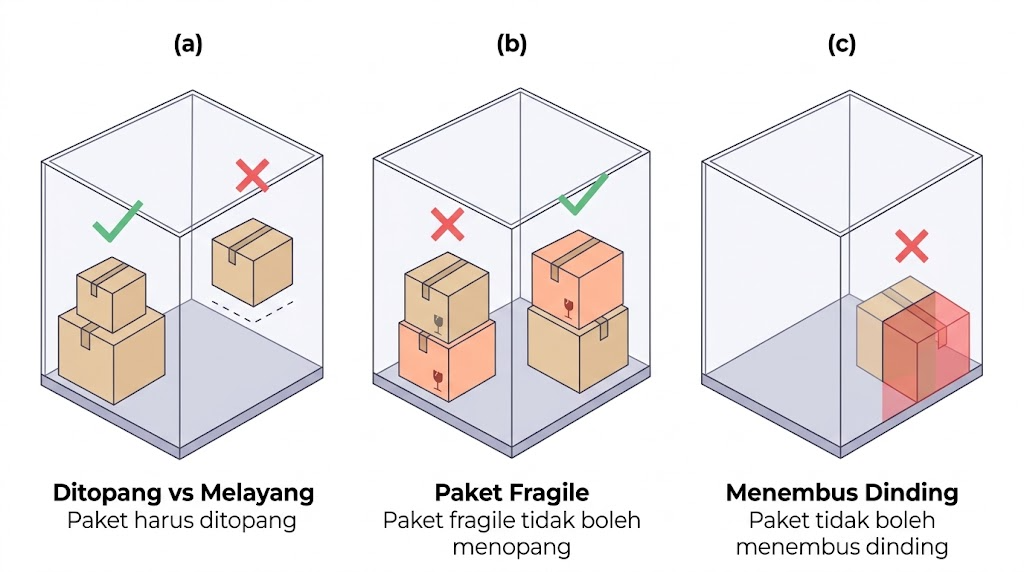
\includegraphics[width=0.75\textwidth]{ilustrasi_constraint.png}}
\caption{Ilustrasi pelanggaran constraint pada penempatan paket\\
(Sumber: dihasilkan dengan Google Gemini)}\label{fig:constraint}
\end{figure}

\section{Ketentuan Pencarian}
Seluruh koordinat bernilai bilangan bulat dan \textit{initial state} dibangkitkan secara acak.
\textit{Neighbor state} dibentuk dengan satu dari tiga jenis \textit{move}: menukar dua paket,
memindahkan satu paket ke koordinat lain, atau merotasi satu paket sebesar $90^\circ$ terhadap
sumbu $x$, $y$, atau $z$. Algoritma yang diminta adalah Hill-Climbing (Steepest Ascent,
Sideways Move, Random Restart, dan Stochastic), Simulated Annealing, dan Genetic Algorithm.

\begin{figure}[H]
\centering
\fbox{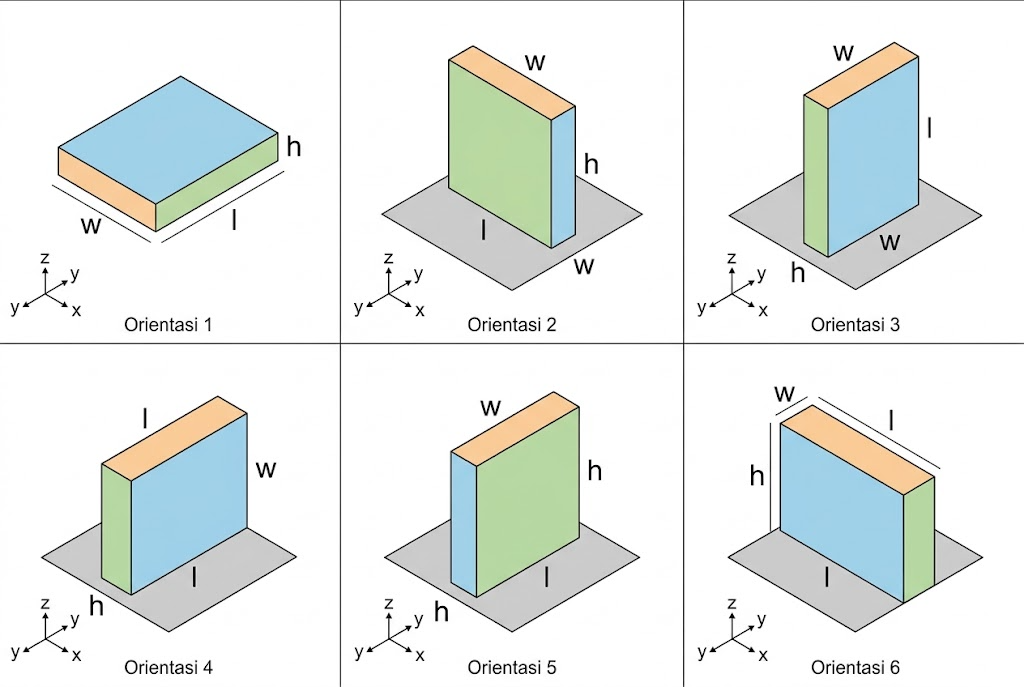
\includegraphics[width=0.75\textwidth]{ilustrasi_orientasi.png}}
\caption{Enam kemungkinan orientasi sebuah paket\\
(Sumber: dihasilkan dengan Google Gemini)}\label{fig:orientasi}
\end{figure}

% =====================================================================
\chapter{LANDASAN TEORI}
% =====================================================================

\section{Local Search}
\textit{Local search} bekerja dengan memegang satu state (atau sekumpulan kecil state) dan
memperbaikinya secara bertahap dengan berpindah ke state tetangga. Berbeda dengan pencarian
klasik seperti BFS atau A*, jalur menuju solusi tidak disimpan karena yang dicari hanyalah
konfigurasi akhirnya \cite{khodra1}.

Kebutuhan memori \textit{local search} sangat kecil dan algoritma ini mampu memberikan solusi
yang cukup baik dalam waktu wajar, sehingga cocok untuk ruang state berukuran besar seperti
penempatan paket tiga dimensi. Konsekuensinya, solusi optimal global tidak dijamin ditemukan.

\section{State, Neighbor, dan Objective Function}
Local search tersusun atas tiga komponen \cite{khodra2}:
\begin{itemize}[leftmargin=1.5cm]
  \item \textbf{State}: satu konfigurasi lengkap dari persoalan.
  \item \textbf{Neighbor}: state lain yang dapat dicapai dengan satu perubahan kecil.
  \item \textbf{Objective function}: fungsi yang memberi skor pada sebuah state; pada persoalan
        maksimasi, skor yang lebih tinggi lebih baik.
\end{itemize}
Seluruh state beserta skornya membentuk \textit{state-space landscape}. Beberapa bentuk landscape
yang menyulitkan pencarian adalah \textit{local maximum} (puncak lokal yang bukan puncak global),
\textit{plateau} atau \textit{shoulder} (daerah datar), dan \textit{ridge} (deretan puncak lokal yang
sulit dilalui dengan satu langkah).

\section{Hill-Climbing}
Hill-Climbing selalu bergerak ke neighbor yang lebih baik dan berhenti ketika tidak ada lagi
neighbor yang lebih baik \cite{khodra3}. Sifatnya yang \textit{greedy} membuat algoritma ini cepat,
tetapi mudah tersangkut di local maximum, plateau, atau ridge. Tabel~\ref{tab:varianhc} merangkum
varian yang dipakai.

\begin{table}[H]
\centering
\caption{Varian Hill-Climbing}\label{tab:varianhc}
\small
\begin{tabular}{|L{3cm}|L{5.6cm}|L{4.6cm}|}
\hline
\hd{Varian} & \hd{Prinsip} & \hd{Berhenti ketika} \\ \hline
Steepest Ascent & Memeriksa seluruh neighbor dan pindah ke yang terbaik & Tidak ada neighbor yang lebih baik \\ \hline
Sideways Move & Seperti Steepest Ascent, tetapi boleh pindah ke neighbor bernilai sama & Langkah datar berturut-turut mencapai batas \\ \hline
Stochastic & Memilih secara acak salah satu neighbor yang lebih baik & Tidak ada neighbor yang lebih baik atau iterasi habis \\ \hline
Random Restart & Mengulang Hill-Climbing dari initial state acak dan menyimpan hasil terbaik & Jumlah restart mencapai batas \\ \hline
\end{tabular}
\end{table}

\section{Simulated Annealing}
Simulated Annealing meniru proses pendinginan logam secara perlahan agar strukturnya stabil
\cite{khodra4}. Pada setiap iterasi dipilih satu neighbor acak. Neighbor yang lebih baik selalu
diterima, sedangkan neighbor yang lebih buruk diterima dengan peluang
\[
P = e^{\Delta E / T},
\]
dengan $\Delta E \le 0$ adalah selisih objective neighbor terhadap state saat ini dan $T$ adalah
suhu. Saat $T$ tinggi, peluang menerima langkah buruk besar sehingga algoritma leluasa
menjelajah. Seiring suhu turun menurut \textit{cooling schedule}, peluang tersebut mengecil dan
perilaku algoritma makin mirip Hill-Climbing.

\section{Genetic Algorithm}
Genetic Algorithm adalah algoritma berbasis populasi yang meniru seleksi alam \cite{khodra5}.
Setiap individu mewakili satu state dan kualitasnya diukur dengan \textit{fitness function}.
Alurnya adalah:
\begin{enumerate}[leftmargin=1.5cm]
  \item membangkitkan populasi awal secara acak;
  \item memilih induk dengan peluang yang sebanding dengan fitness;
  \item melakukan \textit{crossover} untuk menggabungkan informasi dua induk;
  \item melakukan \textit{mutasi} kecil untuk menjaga keragaman;
  \item membentuk generasi baru dan mengulang langkah 2--4 sampai jumlah generasi tercapai.
\end{enumerate}
Ukuran populasi dan jumlah generasi merupakan dua parameter utama: keduanya memperluas
eksplorasi, tetapi juga menambah waktu komputasi.

\section{Penanganan Constraint dengan Fungsi Penalti}
Fungsi penalti memungkinkan algoritma mengunjungi state yang tidak valid dengan cara
mengurangi objective sebesar bobot penalti dikali besar pelanggaran. Apabila bobot penalti lebih
besar daripada nilai maksimum yang mungkin dicapai, setiap state valid pasti lebih baik daripada
setiap state tidak valid. Landscape tetap tersambung, sehingga pencarian tidak terputus hanya
karena satu langkah menghasilkan state tidak valid.

% =====================================================================
\chapter{METODOLOGI}
% =====================================================================

\section{Tahapan Pengerjaan}
Pengerjaan dibagi menjadi enam tahap:
\begin{enumerate}[leftmargin=1.5cm]
  \item Membaca spesifikasi dan merumuskan komponen, constraint, serta tujuan persoalan.
  \item Merancang representasi state, objective, dan operator neighbor yang dipakai bersama oleh ketiga algoritma.
  \item Mengimplementasikan modul inti di \code{src/models/}.
  \item Mengimplementasikan algoritma di \code{src/algoritma/}, program utama \code{main.py}, dan visualisasi di \code{src/visualisasi/}.
  \item Menjalankan eksperimen pada dataset wajib \code{test\_case} dengan seed 1, 2, dan 3.
  \item Menganalisis dan membandingkan hasil.
\end{enumerate}

\section{Representasi Persoalan}
\subsection{Model Data}
Data yang tidak pernah berubah (atribut truk dan paket) dipisahkan dari data yang diubah oleh
algoritma (posisi, orientasi, dan truk tujuan setiap paket). Dengan pemisahan ini, penyalinan
state saat membangkitkan neighbor cukup menyalin bagian yang berubah saja.

\begin{table}[H]
\centering
\caption{Kelas pada model data}\label{tab:kelas}
\small
\begin{tabular}{|L{2.4cm}|L{8cm}|C{2.8cm}|}
\hline
\hd{Kelas} & \hd{Isi} & \hd{Diubah algoritma?} \\ \hline
\code{Truck} & Dimensi $(W, L, H)$ dan \code{max\_capacity} & Tidak \\ \hline
\code{Package} & \code{id}, dimensi asli $(w, l, h)$, \code{value}, \code{weight}, \code{is\_fragile}, \code{eta} & Tidak \\ \hline
\code{Placement} & Referensi \code{Package}, \code{position} $(x,y,z)$ atau \code{None} jika di luar truk, \code{orientation\_idx} (0--5), dan \code{truck\_idx} & Ya \\ \hline
\code{State} & Daftar \code{Truck} dan satu \code{Placement} untuk setiap paket & Ya \\ \hline
\end{tabular}
\end{table}

Paket di luar truk ditandai dengan \code{position = None}. Dengan representasi ini, tidak ada
keadaan ``setengah di dalam'': paket yang koordinatnya menembus dinding dihitung sebagai
pelanggaran, bukan sebagai paket di luar truk. Koordinat $(x, y, z)$ menyatakan sudut
kiri-bawah-belakang paket setelah orientasi diterapkan, dengan titik $(0,0,0)$ di pojok truk.
Sumbu $x$ sejajar $W$, sumbu $y$ sejajar $L$, dan sumbu $z$ sejajar $H$. Pada kasus multi-truk,
setiap truk memiliki sistem koordinat sendiri.

\subsection{Orientasi dan Rotasi}
Orientasi direpresentasikan sebagai permutasi dimensi asli paket ke sumbu $(x, y, z)$, sehingga
terdapat enam orientasi (Tabel~\ref{tab:orientasi}).

\begin{table}[H]
\centering
\caption{Enam orientasi paket}\label{tab:orientasi}
\small
\begin{tabular}{|C{1.6cm}|C{2.6cm}|C{4cm}|C{4cm}|}
\hline
\hd{Indeks} & \hd{Permutasi} & \hd{Dimensi efektif $(x,y,z)$} & \hd{Label} \\ \hline
0 & (0, 1, 2) & $(w, l, h)$ & \{w:x, l:y, h:z\} \\ \hline
1 & (0, 2, 1) & $(w, h, l)$ & \{w:x, l:z, h:y\} \\ \hline
2 & (1, 0, 2) & $(l, w, h)$ & \{w:y, l:x, h:z\} \\ \hline
3 & (1, 2, 0) & $(l, h, w)$ & \{w:z, l:x, h:y\} \\ \hline
4 & (2, 0, 1) & $(h, w, l)$ & \{w:y, l:z, h:x\} \\ \hline
5 & (2, 1, 0) & $(h, l, w)$ & \{w:z, l:y, h:x\} \\ \hline
\end{tabular}
\end{table}

Rotasi $90^\circ$ terhadap sebuah sumbu sama dengan menukar dua komponen permutasi yang tegak
lurus terhadap sumbu tersebut: rotasi terhadap $x$ menukar $y \leftrightarrow z$, terhadap $y$
menukar $x \leftrightarrow z$, dan terhadap $z$ menukar $x \leftrightarrow y$. Keenam orientasi
dapat dicapai dari orientasi mana pun melalui rangkaian rotasi tersebut.

\subsection{Pengecekan Constraint}
Setiap constraint diperiksa per truk, sehingga paket di truk berbeda tidak pernah dianggap
beririsan atau saling menopang.

\begin{table}[H]
\centering
\caption{Definisi pengecekan constraint}\label{tab:constraint}
\small
\begin{tabular}{|L{3cm}|L{7.4cm}|L{2.8cm}|}
\hline
\hd{Constraint} & \hd{Definisi dalam kode} & \hd{Satuan pelanggaran} \\ \hline
Dinding (\code{bounds}) & $x,y,z \ge 0$ dan $x+w \le W$, $y+l \le L$, $z+h \le H$ & Per paket \\ \hline
Overlap & Irisan \textit{axis-aligned bounding box} positif pada ketiga sumbu; bersentuhan sisi tidak dihitung & Per pasangan \\ \hline
Kapasitas (\code{weight}) & $\sum$ berat paket di truk $k \le$ kapasitas truk $k$ & Per truk \\ \hline
Fragile & Ada paket yang alasnya tepat di atap paket fragile dan irisan bidang $xy$ keduanya positif & Per pasangan \\ \hline
Melayang (\code{support}) & Paket dengan $z > 0$ wajib punya minimal satu titik alas di atas atap paket non-fragile & Per paket \\ \hline
\end{tabular}
\end{table}

Paket fragile diperlakukan konsisten di dua tempat: tidak boleh ada paket di atasnya
(constraint fragile) dan tidak dihitung sebagai penopang saat pengecekan melayang.

\section{Fungsi Objektif}
\subsection{Fungsi Objektif Utama}
\[
value(s) = \sum_{i \,\in\, \text{dalam truk}} value_i
\]
Nilai ini tidak memperhitungkan validitas. Validitas ditangani berbeda oleh setiap algoritma
(Tabel~\ref{tab:invalid}).

\begin{table}[H]
\centering
\caption{Penanganan state tidak valid}\label{tab:invalid}
\small
\begin{tabular}{|L{4.5cm}|L{8.7cm}|}
\hline
\hd{Algoritma} & \hd{Penanganan} \\ \hline
Hill-Climbing & Hanya neighbor valid yang dipertimbangkan, sehingga objective cukup $value(s)$ \\ \hline
Simulated Annealing dan Genetic Algorithm & State tidak valid boleh dikunjungi dengan objective berpenalti (subbab~\ref{sub:penalti}) \\ \hline
\end{tabular}
\end{table}

\subsection{Objective Berpenalti (SA dan GA)}\label{sub:penalti}
\begin{align*}
P(s) &= V_{bounds} + V_{overlap} + V_{support} + V_{fragile} + V_{weight} \\
V_{weight} &= \sum_{k\,\in\,\text{truk overload}} \left(1 + \frac{berat_k - kapasitas_k}{kapasitas_k}\right) \\
objective(s) &= value(s) - \lambda \cdot P(s), \qquad \lambda = \sum_{\text{semua paket}} value_i + 1
\end{align*}
\begin{itemize}[leftmargin=1.5cm]
  \item $V_{bounds}$ dan $V_{support}$ dihitung per paket, sedangkan $V_{overlap}$ dan $V_{fragile}$ per pasangan paket.
  \item $\lambda$ lebih besar daripada value maksimum, sehingga state valid apa pun selalu lebih baik daripada state tidak valid.
  \item Di antara state tidak valid, pelanggaran yang lebih sedikit memberi objective lebih tinggi sehingga pencarian punya arah kembali ke daerah valid.
  \item $V_{weight}$ berbentuk pecahan agar pengurangan kelebihan berat tetap dihargai sebagai perbaikan.
\end{itemize}
Karena SA dan GA boleh mengunjungi state tidak valid, kedua algoritma menyimpan dua state hasil:
\begin{itemize}[leftmargin=1.5cm]
  \item \code{final\_state}: pada SA, state tempat pencarian berhenti; pada GA, individu dengan
        fitness berpenalti tertinggi sepanjang run.
  \item \code{best\_valid\_state} (disingkat \code{best\_valid}): state valid dengan value tertinggi
        yang pernah ditemui selama pencarian.
\end{itemize}
Perbandingan kualitas solusi antaralgoritma memakai \code{best\_valid}, sedangkan
\code{final\_state} tetap disimpan untuk menunjukkan kondisi algoritma di akhir pencarian.
Keduanya bisa berbeda. Contohnya, SA seed 1 pada test\_case memiliki \code{final\_state} bernilai
200, tetapi pernah menemukan state valid bernilai 205 (Tabel~\ref{tab:hasilsa}).

\subsection{Fungsi Objektif Bonus: Prioritas ETA}
\[
score_{eta}(s) = \sum_{i \,\in\, \text{dalam truk}} value_i \times \left(1 + \frac{1}{ETA_i}\right)
\]
Paket dengan ETA kecil mendapat bobot lebih besar (2 untuk ETA = 1, 1,5 untuk ETA = 2). Paket
dengan ETA kosong atau tidak positif diberi bobot 1. Saat OF ini dipilih, $\lambda$ disesuaikan
menjadi $\sum score_{eta}$ seluruh paket $+ 1$ dan hasil disimpan terpisah di \code{output/objective\_eta/}.

\section{Initial State dan Neighbor}
\subsection{Initial State}
Initial state dibangkitkan dengan mengacak urutan paket. Untuk setiap paket dicoba hingga 100
kombinasi acak (orientasi, truk, dan posisi di dalam dinding). Penempatan pertama yang menjaga
state tetap valid langsung dipakai; jika seluruh percobaan gagal, paket diletakkan di luar truk.
Oleh karena itu initial state selalu valid, yang merupakan syarat Hill-Climbing.

\subsection{Neighbor Acak (SA dan Mutasi GA)}
Fungsi \code{make\_random\_neighbor} memilih satu dari tiga move dengan peluang sama.

\begin{table}[H]
\centering
\caption{Operator neighbor}\label{tab:move}
\small
\begin{tabular}{|L{2.4cm}|L{10.8cm}|}
\hline
\hd{Move} & \hd{Efek} \\ \hline
Swap & Menukar posisi, orientasi, dan truk dua paket acak (termasuk paket dalam dengan paket luar, atau antartruk) \\ \hline
Relocate & 15\%: paket dikeluarkan dari truk; 85\%: paket dipindah ke truk dan posisi acak di dalam dinding \\ \hline
Rotate & Merotasi satu paket $90^\circ$ terhadap sumbu acak \\ \hline
\end{tabular}
\end{table}
Jika hanya ada satu paket, swap tidak mungkin dilakukan sehingga move diganti menjadi rotate.

\subsection{Seluruh Neighbor (Semua Varian HC)}
Fungsi \code{iter\_all\_feasible\_neighbors} membangkitkan seluruh successor valid dari satu move:
swap untuk setiap pasangan paket ($n(n-1)/2$ kandidat), relocate setiap paket ke luar truk dan ke
setiap koordinat bulat yang muat, serta rotate setiap paket terhadap tiga sumbu ($3n$ kandidat).
Kandidat yang sama dengan state asal atau duplikat (dicek dengan \code{state\_signature})
dibuang. Generator ini dipakai oleh keempat varian HC, termasuk Stochastic.

Seluruh keacakan memakai satu objek \code{random.Random(seed)}, sehingga seed yang sama selalu
menghasilkan run yang sama.

\section{Algoritma}
\subsection{Hill-Climbing}
Keempat varian hanya berpindah ke neighbor valid dengan objective $value(s)$ (atau
$score_{eta}$ jika OF bonus dipilih).

\begin{table}[H]
\centering
\caption{Varian Hill-Climbing yang diimplementasikan}\label{tab:hcimpl}
\small
\begin{tabular}{|L{2.2cm}|L{4.4cm}|L{3.2cm}|L{3.4cm}|}
\hline
\hd{Varian} & \hd{Langkah per iterasi} & \hd{Kondisi berhenti} & \hd{Parameter} \\ \hline
Steepest Ascent & Mengevaluasi seluruh neighbor valid dan pindah ke yang terbaik; seri dipecah acak (\textit{reservoir sampling}) & \code{LOCAL\_OPTIMUM}, \code{NO\_FEASIBLE\_\allowbreak NEIGHBOR}, atau \code{max\_iter} & \code{max\_iter} = 1000 \\ \hline
Sideways Move & Seperti Steepest Ascent, tetapi neighbor terbaik yang bernilai sama juga diterima & \code{MAX\_SIDEWAYS}, \code{LOCAL\_OPTIMUM}, atau \code{max\_iter} & \code{max\_iter} = 1000, \code{max\_consecutive\_\allowbreak sideways} = 50 \\ \hline
Stochastic & Mengumpulkan semua neighbor yang lebih baik (\textit{uphill}) lalu memilih satu secara acak seragam & \code{LOCAL\_OPTIMUM} atau \code{max\_iter} & \code{max\_iter} = 1000 \\ \hline
Random Restart & Steepest Ascent dari initial state, lalu diulang dari initial state acak baru; hasil terbaik disimpan & \code{MAX\_RESTARTS} atau \code{ALL\_PACKAGES\_\allowbreak LOADED} & \code{max\_iter\_\allowbreak per\_\allowbreak restart} = 1000, \code{max\_restart} = 10 \\ \hline
\end{tabular}
\end{table}

Pada Sideways Move, penghitung langkah datar di-\textit{reset} setiap kali terjadi langkah naik,
sehingga yang dibatasi adalah langkah datar berturut-turut. Pada Random Restart, pencarian awal
(dari initial state yang diberikan) dicatat terpisah sebagai \code{initial\_search} dengan label
restart 0, sedangkan \code{restart\_count} hanya menghitung restart sesungguhnya (maksimal 10).

\subsection{Simulated Annealing}
\begin{lstlisting}[mathescape]
current $\leftarrow$ initial_state
untuk t = 0, 1, 2, ...:
    T $\leftarrow$ T0 $\cdot$ $\alpha^t$                  (pendinginan geometrik)
    jika T < T_min atau t $\ge$ max_iter: berhenti
    neighbor $\leftarrow$ neighbor acak, diulang maks max_neighbor_tries kali sampai valid
    $\Delta$E $\leftarrow$ objective(neighbor) - objective(current)
    jika $\Delta$E > 0: terima
    jika $\Delta$E $\le$ 0: terima jika random() < e^($\Delta$E/T)
    jika diterima: current $\leftarrow$ neighbor; perbarui best_valid
    stuck: +1 setiap stuck_window iterasi berturut-turut tanpa objective terbaik naik
\end{lstlisting}

Penerimaan langkah buruk bersifat probabilistik sesuai materi kuliah: langkah turun diterima jika bilangan acak
$r \in [0,1)$ lebih kecil dari $e^{\Delta E/T}$. Untuk $\Delta E > 0$ peluang dicatat sebagai 1, dan
eksponen di atas 709 dibatasi agar tidak terjadi \textit{overflow}.

\begin{table}[H]
\centering
\caption{Parameter Simulated Annealing}\label{tab:paramsa}
\small
\begin{tabular}{|L{4.2cm}|C{2cm}|L{7cm}|}
\hline
\hd{Parameter} & \hd{Nilai} & \hd{Keterangan} \\ \hline
\code{initial\_temperature} ($T_0$) & 100 & Suhu awal \\ \hline
\code{cooling\_rate} ($\alpha$) & 0,999 & Faktor pendinginan geometrik \\ \hline
\code{min\_temperature} & 0,01 & SA selalu berhenti di iterasi ke-9.206 karena suhu \\ \hline
\code{max\_iter} & 20.000 & Tidak pernah tercapai dengan parameter di atas \\ \hline
\code{stuck\_window} & 500 & Panjang jendela tanpa perbaikan \\ \hline
\code{max\_neighbor\_tries} & 50 & Batas percobaan mencari neighbor valid \\ \hline
\end{tabular}
\end{table}

Selain \code{stuck\_count}, dicatat juga \code{stuck\_rate}, yaitu jumlah kejadian stuck per
1.000 iterasi, agar frekuensi stuck dapat dibandingkan antar-run yang panjangnya berbeda.

\subsection{Genetic Algorithm}
Setiap individu adalah satu \code{State} lengkap. Kromosomnya adalah daftar \code{Placement}
dengan satu gen per paket, dan setiap gen berisi posisi, orientasi, serta truk paket tersebut.
Fitness memakai objective berpenalti yang sama dengan SA (subbab~\ref{sub:penalti}), sehingga
individu tidak valid tetap boleh ada di populasi tetapi hampir tidak pernah mengalahkan individu
valid. Alur satu generasi adalah sebagai berikut.
\begin{enumerate}[leftmargin=1.5cm]
  \item \textbf{Evaluasi}: fitness seluruh individu dihitung, lalu individu terbaik dan
        \code{best\_valid} diperbarui.
  \item \textbf{Elitisme}: \code{elitisme} = 2 individu dengan fitness tertinggi disalin langsung ke
        generasi berikutnya.
  \item \textbf{Seleksi}: dua induk dipilih dengan \textit{roulette wheel}. Fitness digeser terhadap
        nilai minimum populasi agar semua bobot positif, karena fitness berpenalti bisa negatif.
  \item \textbf{Crossover}: dengan peluang \code{crossover\_rate} = 0,81 dilakukan
        \textit{uniform crossover}: untuk setiap paket, gen diambil dari induk pertama atau kedua
        dengan peluang masing-masing 0,5. Gen dicocokkan berdasarkan \code{id} paket, sehingga anak
        selalu berisi tepat satu placement untuk setiap paket. Jika crossover tidak terjadi, anak
        adalah salinan induk pertama.
  \item \textbf{Mutasi}: dengan peluang \code{mutation\_rate} = 0,2, anak dikenai 1--3 move acak dari
        \code{make\_random\_neighbor} (swap, relocate, atau rotate).
  \item Langkah 3--5 diulang sampai ukuran populasi kembali penuh.
\end{enumerate}

GA tidak memiliki kriteria berhenti dini. Pencarian selalu berjalan tepat \code{max\_iter}
generasi, sehingga jumlah populasi dan iterasi menjadi parameter yang diuji pada eksperimen.

\begin{table}[H]
\centering
\caption{Parameter Genetic Algorithm}\label{tab:paramga}
\small
\begin{tabular}{|L{4.2cm}|C{2.6cm}|L{6.4cm}|}
\hline
\hd{Parameter} & \hd{Nilai} & \hd{Keterangan} \\ \hline
\code{population\_size} & 20 / 50 / 100 & Divariasikan pada eksperimen B (iterasi 100) \\ \hline
\code{max\_iter} & 50 / 100 / 200 & Jumlah generasi; divariasikan pada eksperimen A (populasi 50) \\ \hline
\code{crossover\_rate} & 0,81 & Peluang crossover per pasangan induk \\ \hline
\code{mutation\_rate} & 0,2 & Peluang seorang anak dimutasi \\ \hline
\code{mutation\_moves} & 3 & Batas atas jumlah move per mutasi (nilai bawaan, tidak diatur di \code{experiments.json}) \\ \hline
\code{elitisme} & 2 & Individu terbaik yang dibawa tanpa perubahan \\ \hline
\end{tabular}
\end{table}

Ada dua hasil yang disimpan. \code{final\_state} adalah individu dengan fitness berpenalti
tertinggi sepanjang run, dan \code{initial\_state} adalah individu terbaik generasi 0. Hasil yang
dilaporkan adalah \code{best\_valid}, yaitu individu valid dengan value tertinggi yang pernah muncul.
Jika \code{max\_iter} = 0, loop tidak berjalan dan GA langsung mengambil individu terbaik dari
populasi awal.

\subsection{Bonus Multi-Truk}
Multi-truk ditangani di tingkat representasi, bukan di tingkat algoritma. Setiap
\code{Placement} menyimpan \code{truck\_idx}, dan setiap truk memiliki sistem koordinat sendiri.
Dukungan multi-truk tersebar pada komponen berikut:
\begin{itemize}[leftmargin=1.5cm]
  \item \textbf{Dataset}: \code{load\_dataset} menerima format satu truk (\code{"truck"}) maupun
        daftar truk (\code{"trucks"}); format satu truk diperlakukan sebagai daftar berisi satu truk.
  \item \textbf{Initial state}: setiap percobaan penempatan memilih truk secara acak.
  \item \textbf{Neighbor acak}: relocate memilih truk tujuan secara acak, sedangkan swap ikut
        menukar \code{truck\_idx} sehingga dua paket dapat bertukar truk.
  \item \textbf{Seluruh neighbor (HC)}: relocate mencoba setiap koordinat di \emph{setiap} truk yang
        cukup besar untuk paket tersebut.
  \item \textbf{Constraint}: overlap, fragile, dan support hanya diperiksa antarpaket pada truk yang
        sama, sedangkan kapasitas dihitung per truk terhadap \code{max\_capacity} masing-masing.
\end{itemize}
Karena itu HC, SA, dan GA dapat menyelesaikan kasus multi-truk tanpa perubahan kode algoritma.
Sebagai uji coba, GA dijalankan pada \code{multi\_truck\_case} (dua truk, kapasitas 100 dan 80,
dengan delapan paket yang sama seperti \code{test\_case}). Dengan populasi 10 dan 10 iterasi, GA
memperoleh value 305, yang berarti seluruh paket berhasil dimuat ke dua truk.

\section{Heuristik yang Digunakan}
\begin{itemize}[leftmargin=1.5cm]
  \item \textbf{Initial state selalu valid.} Paket hanya ditambahkan jika state tetap valid, sehingga
        HC dapat langsung berjalan dan SA/GA mulai dari daerah valid.
  \item \textbf{Mengeluarkan paket saat relocate (15\%).} Pada neighbor acak, relocate memiliki
        peluang 15\% untuk mengeluarkan paket dari truk. Langkah ini membuka ruang bagi paket lain
        ketika susunan sudah terkunci.
  \item \textbf{Neighbor duplikat dibuang.} Dalam satu neighborhood, kandidat yang sama dengan state
        asal atau dengan kandidat sebelumnya (dicek dengan \code{state\_signature}) tidak dievaluasi
        ulang. Pengecekan ini hanya berlaku dalam satu iterasi, sehingga Sideways Move tetap dapat
        kembali ke state yang pernah dikunjungi; yang membatasinya adalah
        \code{max\_consecutive\_sideways}.
  \item \textbf{Seri dipecah secara acak.} Jika beberapa neighbor terbaik bernilai sama, salah satunya
        dipilih acak dengan \textit{reservoir sampling}, sehingga HC tidak selalu bergerak ke arah
        yang sama.
  \item \textbf{Bobot penalti $\lambda$ = total value + 1.} State valid apa pun selalu lebih baik
        daripada state tidak valid, tetapi state tidak valid masih dapat dibandingkan berdasarkan
        banyaknya pelanggaran.
  \item \textbf{Penalti berat berbentuk pecahan.} Mengurangi kelebihan berat tetap dihargai sebagai
        perbaikan walaupun truk belum berada di bawah kapasitas.
  \item \textbf{Neighbor valid untuk SA.} SA mencoba hingga \code{max\_neighbor\_tries} = 50 kali untuk
        mendapatkan neighbor valid. Pada test\_case, state current SA tetap valid di seluruh iterasi.
  \item \textbf{Penyimpanan \code{best\_valid}.} Solusi bagus yang sempat ditinggalkan SA pada suhu
        tinggi, atau yang hilang di GA akibat crossover, tetap tersimpan sebagai hasil.
\end{itemize}

% =====================================================================
\chapter{PERANCANGAN \& IMPLEMENTASI}
% =====================================================================

\section{Struktur Program}
Program ditulis dalam Python dengan satu dependensi eksternal, yaitu \code{matplotlib} untuk
visualisasi. Kode terbagi menjadi modul inti yang dipakai bersama, algoritma, serta program utama
dan visualisasi.

\begin{figure}[H]
\centering
\begin{lstlisting}[frame=single]
src/
  main.py               # program utama (menu CLI)
  models/
    model.py            # Package, Truck, Placement, State, orientasi
    geometry.py         # pengecekan lima constraint
    objective.py        # OF value dan OF bonus eta
    operators.py        # initial state dan operator neighbor
    io.py               # baca dataset, simpan/muat state, history, config
  algoritma/
    HC.py               # empat varian Hill-Climbing
    SA.py               # Simulated Annealing
    GA.py               # Genetic Algorithm
  visualisasi/
    plots.py            # plot objective, e^(dE/T), dan state 3D
    export_replay.py    # rekam state per langkah untuk viewer
    viewer3d.html       # viewer 3D interaktif (Three.js)
  data/                 # dataset dan experiments.json
tests/
  test_hc.py  test_sa.py  test_ga.py
\end{lstlisting}
\caption{Struktur direktori program}
\end{figure}

HC dan SA menerima \code{run(initial\_state, rng, **params)}, sedangkan GA menerima
\code{run(trucks, packages, rng, population\_size, max\_iter, **params)} karena GA membangkitkan
populasinya sendiri. Ketiganya mengembalikan \code{dict} dengan kunci yang seragam
(\code{initial\_state}, \code{final\_state}, \code{best\_valid\_state}, \code{final\_objective},
\code{iterations}, \code{duration\_s}, \code{history}, \code{extra}), sehingga penyimpanan hasil
dan visualisasi dapat dipakai bersama. Parameter eksperimen dibaca dari \code{data/experiments.json}.

\section{Modul Inti (src/models/)}
Modul inti berisi model data, pengecekan constraint, fungsi objektif, operator neighbor, dan I/O
yang dipakai bersama oleh ketiga algoritma.

\subsection{model.py}
\begin{table}[H]
\centering
\caption{Isi model.py}
\small
\begin{tabular}{|L{5.2cm}|L{1.8cm}|L{6.2cm}|}
\hline
\hd{Nama} & \hd{Jenis} & \hd{Deskripsi} \\ \hline
\code{ORIENTATIONS} & Konstanta & Enam permutasi dimensi beserta labelnya \\ \hline
\code{get\_effective\_dimensions} & Fungsi & Dimensi paket pada sumbu $(x,y,z)$ untuk suatu orientasi \\ \hline
\code{rotate\_orientation\_idx} & Fungsi & Indeks orientasi baru setelah rotasi $90^\circ$ \\ \hline
\code{Package}, \code{Truck} & Kelas & Data tetap paket dan truk \\ \hline
\code{Placement} & Kelas & Posisi, orientasi, truk; menyediakan \code{effective\_dims} dan \code{aabb()} \\ \hline
\code{State} & Kelas & Daftar truk dan placement; \code{total\_value()}, \code{truck\_weight()}, \code{copy()}, konversi JSON \\ \hline
\end{tabular}
\end{table}

\begin{lstlisting}[language=Python]
def rotate_orientation_idx(current_idx: int, axis: str) -> int:
    perm = list(ORIENTATIONS[current_idx])
    if axis == "x":
        perm[1], perm[2] = perm[2], perm[1]
    elif axis == "y":
        perm[0], perm[2] = perm[2], perm[0]
    else:  # z
        perm[0], perm[1] = perm[1], perm[0]
    return _PERM_TO_IDX[tuple(perm)]
\end{lstlisting}

\subsection{geometry.py}
\begin{table}[H]
\centering
\caption{Fungsi pada geometry.py}
\small
\begin{tabular}{|L{5cm}|L{8.2cm}|}
\hline
\hd{Fungsi} & \hd{Deskripsi} \\ \hline
\code{is\_inside\_bounds}, \code{check\_bounds} & Constraint dinding \\ \hline
\code{placements\_overlap}, \code{check\_no\_overlap} & Constraint overlap (uji AABB per truk) \\ \hline
\code{check\_weight}, \code{overweight\_score} & Constraint kapasitas dan besar kelebihan berat \\ \hline
\code{check\_fragile\_support} & Constraint paket di atas paket fragile \\ \hline
\code{check\_support} & Constraint melayang \\ \hline
\code{validate}, \code{is\_feasible} & Menjalankan kelima pengecekan dan mengembalikan pelanggaran per kategori \\ \hline
\end{tabular}
\end{table}

Dua balok tidak beririsan jika keduanya terpisah pada minimal satu sumbu. Penggunaan \code{<=}
membuat paket yang hanya bersentuhan sisi tidak dianggap overlap:
\begin{lstlisting}[language=Python]
def placements_overlap(a: Placement, b: Placement) -> bool:
    ax1, ay1, az1, ax2, ay2, az2 = a.aabb()
    bx1, by1, bz1, bx2, by2, bz2 = b.aabb()
    if ax2 <= bx1 or bx2 <= ax1: return False
    if ay2 <= by1 or by2 <= ay1: return False
    if az2 <= bz1 or bz2 <= az1: return False
    return True
\end{lstlisting}

\subsection{objective.py}
Definisi objective dipisahkan dari algoritma, sehingga OF bonus dapat dipakai oleh ketiga
algoritma tanpa mengubah kodenya.
\begin{lstlisting}[language=Python]
def eta_weight(package: Package) -> float:
    if package.eta is None or package.eta <= 0:
        return 1.0
    return 1.0 + 1.0 / package.eta
\end{lstlisting}

\subsection{operators.py}
\begin{table}[H]
\centering
\caption{Fungsi pada operators.py}
\small
\begin{tabular}{|L{5.4cm}|L{7.8cm}|}
\hline
\hd{Fungsi} & \hd{Deskripsi} \\ \hline
\code{make\_initial\_state} & Initial state acak yang selalu valid \\ \hline
\code{swap\_packages}, \code{relocate\_package}, \code{rotate\_package} & Tiga move dasar; mengembalikan salinan state baru \\ \hline
\code{relocate\_random}, \code{rotate\_random} & Versi acak relocate dan rotate \\ \hline
\code{make\_random\_neighbor} & Satu move acak (SA dan mutasi GA) \\ \hline
\code{iter\_all\_feasible\_neighbors} & Generator seluruh neighbor valid unik (semua varian HC) \\ \hline
\code{state\_signature} & Representasi state yang dapat di-\textit{hash} \\ \hline
\end{tabular}
\end{table}

\subsection{io.py}
\code{load\_dataset} membaca dataset satu truk maupun multi-truk, \code{save\_state}/\code{load\_state}
menyimpan dan memuat state, \code{save\_history\_csv} menyimpan riwayat per iterasi, dan
\code{load\_config} membaca \code{experiments.json}.

\section{Implementasi Hill-Climbing (HC.py)}
\begin{table}[H]
\centering
\caption{Fungsi pada HC.py}
\small
\begin{tabular}{|L{4.6cm}|L{8.6cm}|}
\hline
\hd{Fungsi} & \hd{Deskripsi} \\ \hline
\code{run\_steepest} & Steepest Ascent \\ \hline
\code{run\_sideways} & Sideways Move \\ \hline
\code{run\_stochastic} & Stochastic: pilih acak di antara neighbor yang lebih baik \\ \hline
\code{run\_random\_restart} & Random Restart (memanggil \code{run\_steepest} berulang kali) \\ \hline
\code{\_best\_feasible\_neighbor} & Neighbor valid terbaik dari seluruh neighborhood \\ \hline
\end{tabular}
\end{table}

Inti Stochastic Hill-Climbing:
\begin{lstlisting}[language=Python]
uphill = []
for neighbor in iter_all_feasible_neighbors(current):
    value = state_score(neighbor, objective)
    if value > current_value:
        uphill.append((neighbor, value))
if not uphill:
    termination_reason = "LOCAL_OPTIMUM"
    break
current, current_value = uphill[rng.randrange(len(uphill))]
\end{lstlisting}

\section{Implementasi Simulated Annealing (SA.py)}
\begin{table}[H]
\centering
\caption{Fungsi pada SA.py}
\small
\begin{tabular}{|L{4.6cm}|L{8.6cm}|}
\hline
\hd{Fungsi} & \hd{Deskripsi} \\ \hline
\code{penalty} & Jumlah pelanggaran kelima constraint, $P(s)$ \\ \hline
\code{objective\_function} & Objective berpenalti $value(s) - \lambda \cdot P(s)$ \\ \hline
\code{schedule} & Suhu pada iterasi ke-$t$, yaitu $T_0 \cdot \alpha^t$ \\ \hline
\code{acceptance\_probability} & Menghitung $e^{\Delta E/T}$ dengan pengaman \textit{overflow} \\ \hline
\code{make\_valid\_neighbor} & Neighbor acak yang diulang sampai valid, maksimal \code{max\_neighbor\_tries} kali \\ \hline
\code{run} & Loop utama Simulated Annealing \\ \hline
\code{params\_from\_config} & Membaca parameter dari bagian \code{simulated\_annealing} pada \code{experiments.json} \\ \hline
\code{save\_result} & Menyimpan state awal/akhir, \code{history.csv}, dan \code{summary.json} \\ \hline
\end{tabular}
\end{table}

Penalti dan objective berpenalti diimplementasikan langsung dari rumus pada subbab~\ref{sub:penalti}.
Nilai $\lambda$ diambil dari \code{max\_score}, sehingga otomatis menyesuaikan saat OF bonus dipakai:
\begin{lstlisting}[language=Python]
def penalty(state: State) -> float:
    violations = validate(state)
    return (len(violations["bounds"]) + len(violations["overlap"])
            + len(violations["support"]) + len(violations["fragile"])
            + overweight_score(state))

def objective_function(state: State, objective: str = "value") -> float:
    lambda_penalty = max_score(state, objective) + 1
    return state_score(state, objective) - lambda_penalty * penalty(state)
\end{lstlisting}

Suhu turun secara geometrik, dan peluang penerimaan dibatasi agar \code{math.exp} tidak
\textit{overflow} ketika $\Delta E/T$ sangat besar ($e^{709}$ mendekati batas \code{float}):
\begin{lstlisting}[language=Python]
def schedule(iteration, initial_temperature, cooling_rate):
    return initial_temperature * (cooling_rate ** iteration)

def acceptance_probability(delta_e, temperature):
    ratio = delta_e / temperature
    if ratio > 709.0:
        return float("inf")
    return math.exp(ratio)
\end{lstlisting}

Neighbor dicari dengan \code{make\_random\_neighbor} sampai valid. Jika dalam
\code{max\_neighbor\_tries} percobaan tidak ada yang valid, kandidat terakhir tetap dipakai dan
penalti pada objective yang akan membuatnya hampir pasti ditolak:
\begin{lstlisting}[language=Python]
def make_valid_neighbor(state, rng, max_tries):
    for tries in range(1, max_tries + 1):
        neighbor = make_random_neighbor(state, rng)
        if is_feasible(neighbor)[0]:
            break
    return neighbor, tries
\end{lstlisting}

Inti loop \code{run} adalah sebagai berikut. Langkah naik selalu diterima, sedangkan langkah datar
atau turun diterima dengan membandingkan bilangan acak terhadap $e^{\Delta E/T}$:
\begin{lstlisting}[language=Python]
while iteration < max_iter:
    temperature = schedule(iteration, initial_temperature, cooling_rate)
    if temperature < min_temperature:
        break
    neighbor, tries = make_valid_neighbor(current, rng, max_neighbor_tries)
    neighbor_obj = objective_function(neighbor, objective)
    delta_e = neighbor_obj - current_obj

    if delta_e > 0:
        accept_prob = 1.0
        accepted = True
    else:
        accept_prob = acceptance_probability(delta_e, temperature)
        accepted = rng.random() < accept_prob

    if accepted:
        current, current_obj = neighbor, neighbor_obj
        current_feasible = is_feasible(current)[0]
        if current_feasible and (best_valid_state is None or
                state_score(current, objective) > state_score(best_valid_state, objective)):
            best_valid_state = current.copy()
    ...
    iteration += 1
\end{lstlisting}

Frekuensi stuck dihitung di dalam loop yang sama. Penghitung \code{no\_improve\_local} bertambah
setiap iterasi yang tidak memperbaiki objective terbaik. Saat mencapai \code{stuck\_window},
\code{stuck\_count} bertambah satu dan penghitung di-\textit{reset}:
\begin{lstlisting}[language=Python]
if current_obj > best_obj:
    best_obj = current_obj
    no_improve_local = 0
else:
    no_improve_local += 1
    if no_improve_local >= stuck_window:
        stuck_count_global += 1
        no_improve_local = 0
\end{lstlisting}

Setiap iterasi mencatat suhu, objective, value, status valid, $\Delta E$, peluang penerimaan,
status diterima, dan jumlah percobaan neighbor ke \code{history}. Data ini dipakai untuk membuat
\code{objective.png} dan \code{accept\_prob.png}. Setelah loop selesai, \code{stuck\_rate} dihitung
sebagai \code{stuck\_count} per 1.000 iterasi.

\section{Implementasi Genetic Algorithm (GA.py)}
\begin{table}[H]
\centering
\caption{Fungsi pada GA.py}
\small
\begin{tabular}{|L{4.6cm}|L{8.6cm}|}
\hline
\hd{Fungsi} & \hd{Deskripsi} \\ \hline
\code{penalty}, \code{objective\_function} & Fitness berpenalti, sama dengan SA \\ \hline
\code{make\_population} & Populasi awal dari \code{make\_initial\_state} (semua valid) \\ \hline
\code{roulette} & Seleksi \textit{roulette wheel} dengan fitness yang digeser ke positif \\ \hline
\code{crossover} & \textit{Uniform crossover} per paket \\ \hline
\code{mutate} & 1--3 move acak dengan peluang \code{mutation\_rate} \\ \hline
\code{best\_by\_fitness} & Individu dengan fitness tertinggi pada suatu populasi \\ \hline
\code{best\_valid} & Individu valid dengan value tertinggi pada suatu populasi \\ \hline
\code{run} & Loop generasi GA \\ \hline
\code{experiment\_matrix} & Daftar konfigurasi eksperimen A dan B dari \code{experiments.json} \\ \hline
\code{save\_result} & Menyimpan state, \code{history.csv}, dan \code{summary.json} \\ \hline
\end{tabular}
\end{table}

Fitness pada objective berpenalti bisa bernilai negatif, sehingga sebelum seleksi semua nilai
digeser terhadap fitness terkecil. Dengan begitu setiap individu tetap memiliki bobot positif:
\begin{lstlisting}[language=Python]
def roulette(population, fitnesses, rng):
    floor = min(fitnesses)
    weights = [f - floor + 1e-6 for f in fitnesses]
    threshold = rng.random() * sum(weights)
    cumulative = 0.0
    for individual, weight in zip(population, weights):
        cumulative += weight
        if cumulative >= threshold:
            return individual
    return population[-1]
\end{lstlisting}

Kromosom adalah daftar \code{Placement}, satu gen per paket. Crossover memilih gen dari salah
satu induk dengan peluang 0,5 per paket. Karena gen dicocokkan berdasarkan \code{id} paket, anak
selalu berisi tepat satu placement untuk setiap paket. Mutasi memakai operator neighbor yang
sama dengan SA:
\begin{lstlisting}[language=Python]
def crossover(parent_a, parent_b, rng, crossover_rate):
    if rng.random() >= crossover_rate:
        return parent_a.copy()
    donor = {p.package.id: p for p in parent_b.placements}
    child_placements = []
    for placement in parent_a.placements:
        source = placement if rng.random() < 0.5 else donor[placement.package.id]
        child_placements.append(source.copy())
    return State(trucks=list(parent_a.trucks), placements=child_placements)

def mutate(individual, rng, mutation_rate, max_moves=3):
    child = individual.copy()
    if rng.random() >= mutation_rate:
        return child
    for _ in range(rng.randint(1, max_moves)):
        child = make_random_neighbor(child, rng)
    return child
\end{lstlisting}

Pada setiap generasi, \code{run} menghitung fitness, mencatat statistik populasi, memperbarui
individu terbaik dan \code{best\_valid}, lalu membentuk generasi baru. Elitisme dilakukan dengan
menyalin \code{elitisme} individu terbaik terlebih dahulu, kemudian sisa populasi diisi anak hasil
seleksi, crossover, dan mutasi:
\begin{lstlisting}[language=Python]
for iteration in range(max_iter):
    fitnesses = [objective_function(ind, objective) for ind in population]
    values = [ind.total_value() if is_feasible(ind)[0] else 0
              for ind in population]
    # perbarui best_individual dan best_valid_state, catat history
    ...
    if iteration == max_iter - 1:
        break
    elite_indices = sorted(range(len(population)),
                           key=lambda i: fitnesses[i], reverse=True)[:elitisme]
    next_population = [population[i].copy() for i in elite_indices]
    while len(next_population) < population_size:
        parent_a = roulette(population, fitnesses, rng)
        parent_b = roulette(population, fitnesses, rng)
        child = crossover(parent_a, parent_b, rng, crossover_rate)
        child = mutate(child, rng, mutation_rate, mutation_moves)
        next_population.append(child)
    population = next_population
\end{lstlisting}

Setiap generasi mencatat \code{max\_objective}, \code{avg\_objective}, \code{best\_value},
\code{avg\_value} (individu tidak valid dihitung 0), dan \code{feasible\_count}. Kedua panel
\code{objective.png} digambar dari data ini. Individu terbaik generasi 0 disimpan sebagai
\code{initial\_state}, sedangkan individu terbaik sepanjang run disimpan sebagai
\code{final\_state}. Jika \code{max\_iter} = 0, loop tidak berjalan dan GA langsung mengambil
individu terbaik dari populasi awal.

% =====================================================================
\chapter{PENGUJIAN}
% =====================================================================

\section{Skenario Pengujian}
Agar pengujian tetap ringkas, seluruh eksperimen hanya memakai dataset wajib \code{test\_case}
dengan parameter default \code{experiments.json} dan seed 1, 2, 3, sesuai jumlah minimum run yang
diminta spesifikasi. Unit test di folder \code{tests/} dipakai untuk memastikan kebenaran
implementasi.

Seluruh eksperimen dijalankan pada satu perangkat yang sama, yaitu laptop dengan prosesor
Intel Core Ultra 5 125H, RAM 16 GB, sistem operasi Windows 11 Home, dan Python 3.12.0.
Dengan demikian, durasi antaralgoritma dapat dibandingkan secara langsung. Nilai durasi hanya
berlaku relatif terhadap perangkat ini.

\begin{table}[H]
\centering
\caption{Skenario eksperimen}\label{tab:skenario}
\small
\begin{tabular}{|L{3.4cm}|L{6.4cm}|C{3cm}|}
\hline
\hd{Eksperimen} & \hd{Konfigurasi} & \hd{Jumlah run} \\ \hline
HC (4 varian) & Parameter Tabel~\ref{tab:hcimpl} & $4 \times 3 = 12$ \\ \hline
SA & Parameter Tabel~\ref{tab:paramsa} & 3 \\ \hline
GA eksperimen A & Populasi 50; iterasi 50 / 100 / 200 & 9 \\ \hline
GA eksperimen B & Iterasi 100; populasi 20 / 50 / 100 & 9 \\ \hline
\end{tabular}
\end{table}

Alur bilangan acak HC dan SA sama, sehingga untuk setiap seed keempat varian HC dan SA berangkat
dari initial state yang sama, yaitu value 205 (seed 1), 165 (seed 2), dan 135 (seed 3).
GA membangkitkan populasinya sendiri.

\section{Dataset Uji}
\code{test\_case} berisi satu truk berukuran $6 \times 6 \times 4$ dengan kapasitas 100 dan delapan
paket (dua di antaranya fragile, P2 dan P6). Total value seluruh paket 305 dan total beratnya 156.
Batas atas dihitung dengan knapsack 0/1 berbasis berat (kapasitas 100) yang mengabaikan geometri,
menghasilkan 205. Karena constraint geometri hanya dapat menurunkan nilai, state valid bernilai
205 pasti merupakan optimum global.

\section{Data yang Dicatat}
\begin{table}[H]
\centering
\caption{Pemetaan data yang diminta spesifikasi ke output program}
\small
\begin{tabular}{|L{6cm}|L{7.2cm}|}
\hline
\hd{Diminta spesifikasi} & \hd{Lokasi pada output} \\ \hline
State awal dan akhir & \code{initial\_state.json}, \code{final\_state.json}, beserta gambar \\ \hline
Nilai objective akhir & \code{summary.json}: \code{final\_objective}, \code{best\_valid\_value} \\ \hline
Plot objective terhadap iterasi & \code{objective.png} \\ \hline
Durasi & \code{summary.json}: \code{duration\_s} \\ \hline
HC: iterasi sampai berhenti & \code{iterations}, \code{termination\_reason} \\ \hline
HC Sideways: iterasi dan batas sideways & \code{params.max\_consecutive\_sideways}, \code{extra.sideways\_moves} \\ \hline
HC Random Restart: restart dan iterasi per restart & \code{extra.restart\_count}, \code{extra.iterations\_per\_restart}, \code{restart\_summary.csv} \\ \hline
SA: plot $e^{\Delta E/T}$ dan frekuensi stuck & \code{accept\_prob.png}, \code{stuck\_count}, \code{stuck\_rate} \\ \hline
GA: objective maksimum dan rata-rata & \code{objective.png}, \code{history.csv} \\ \hline
\end{tabular}
\end{table}

\section{Hasil pada Test Case}
\subsection{Hill-Climbing}
\begin{table}[H]
\centering
\caption{Hasil Hill-Climbing pada test\_case}\label{tab:hasilhc}
\small
\begin{tabular}{|L{2.3cm}|C{2.5cm}|C{2.2cm}|C{1.6cm}|L{4.4cm}|}
\hline
\hd{Varian} & \hd{Value akhir (seed 1/2/3)} & \hd{Iterasi (seed 1/2/3)} & \hd{Durasi rata-rata (s)} & \hd{Keterangan} \\ \hline
Steepest Ascent & 205 / 190 / 150 & 1 / 2 / 2 & 0,05 & \code{LOCAL\_OPTIMUM} \\ \hline
Sideways Move & 205 / 190 / 185 & 50 / 51 / 54 & 1,82 & \code{MAX\_SIDEWAYS}; total sideways 50 / 50 / 51 \\ \hline
Stochastic & 205 / 190 / 150 & 1 / 3 / 2 & 0,05 & \code{LOCAL\_OPTIMUM}; langkah diterima 0 / 2 / 1 \\ \hline
Random Restart & 205 / 205 / 200 & 12 / 16 / 15 & 0,68 & \code{MAX\_RESTARTS}; 10 restart; restart terbaik 0 / 6 / 5 \\ \hline
\end{tabular}
\end{table}

Pada Sideways Move, \code{max\_consecutive\_sideways} = 50 membatasi jumlah langkah datar
\emph{berturut-turut}, bukan jumlah total langkah datar selama pencarian. Penghitungnya kembali
ke 0 setiap kali terjadi langkah naik. Oleh karena itu total sideways pada seed 3 bisa bernilai 51:
dari 54 iterasi, 3 merupakan langkah naik dan 51 merupakan langkah datar, dengan 50 langkah datar
berturut-turut di bagian akhir.

Dengan \code{max\_restart} = 10, Random Restart menjalankan Steepest Ascent sebanyak 11 kali, yaitu
satu pencarian dari initial state awal dan 10 pencarian dari initial state baru hasil restart.
Iterasi per restart pada Random Restart (di luar pencarian awal) adalah
[2, 1, 1, 1, 1, 1, 1, 1, 1, 1] untuk seed 1, [1, 1, 3, 1, 1, 3, 1, 1, 1, 1] untuk seed 2, dan
[1, 1, 1, 1, 3, 1, 1, 1, 2, 1] untuk seed 3. Pencarian awalnya masing-masing berakhir di 205, 190,
dan 150.

\begin{figure}[H]
\centering
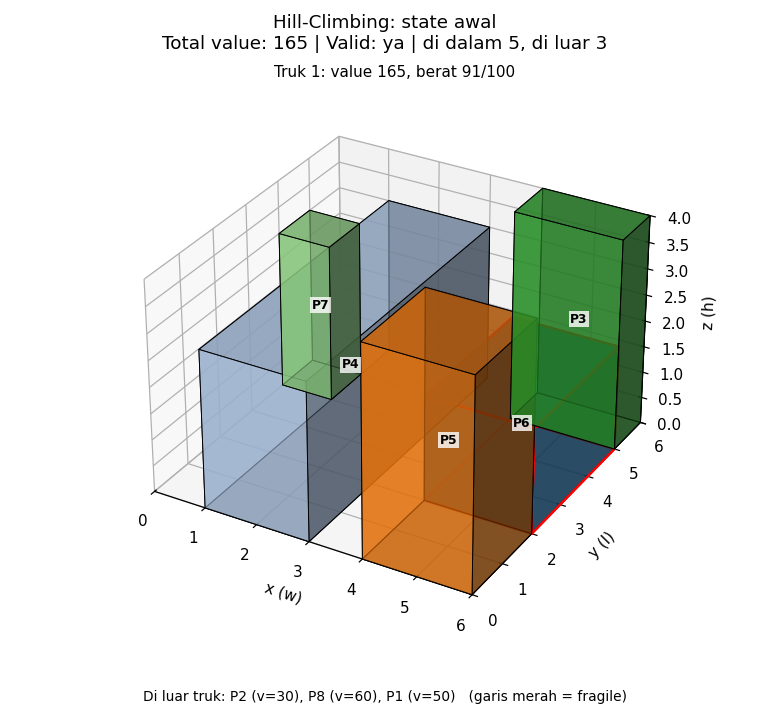
\includegraphics[width=0.75\textwidth]{hc/test_case/steepest_ascent/run2_seed2/initial_state.png}
\caption{State awal test\_case seed 2 (value 165), dipakai bersama oleh keempat varian HC dan SA}
\end{figure}

\begin{figure}[H]
\centering
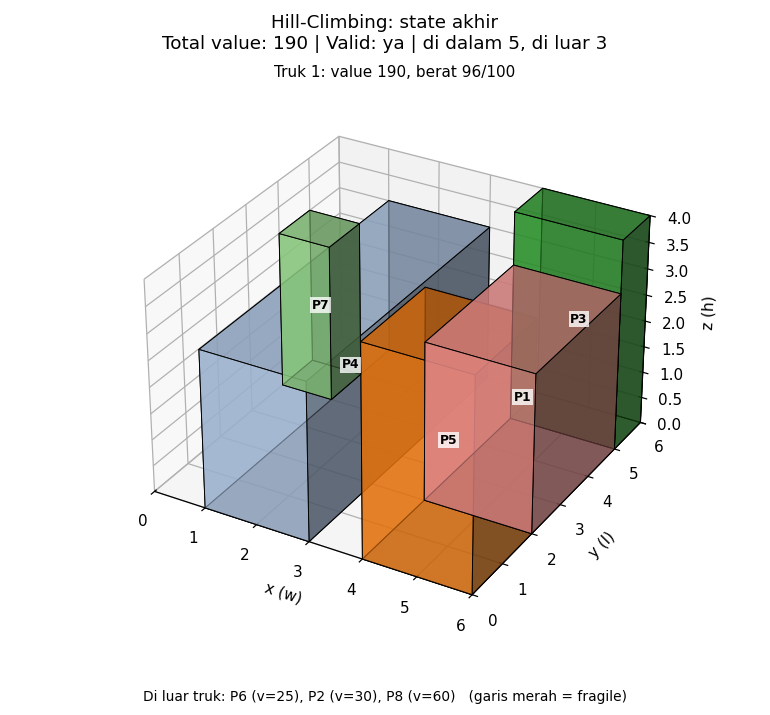
\includegraphics[width=0.48\textwidth]{hc/test_case/steepest_ascent/run2_seed2/final_state.png}\hfill
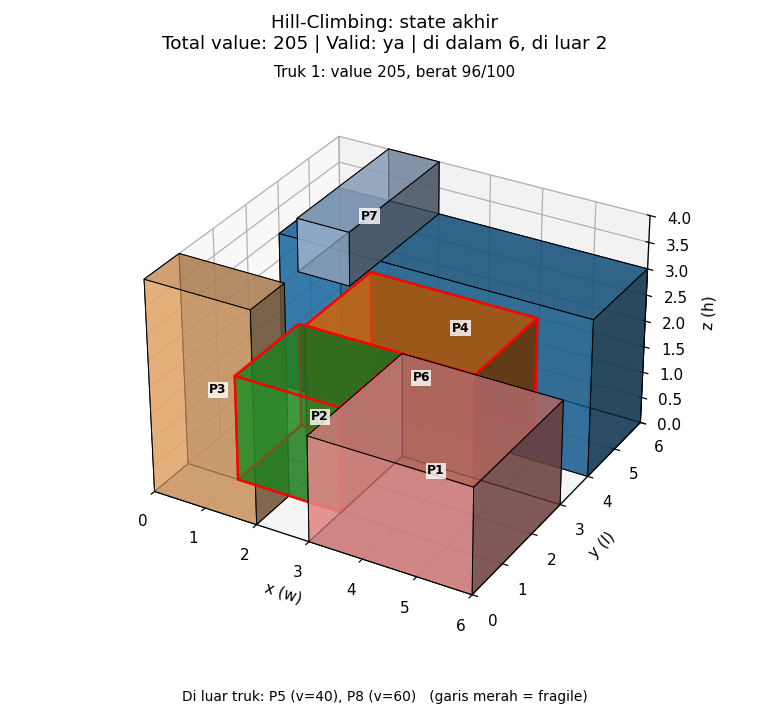
\includegraphics[width=0.48\textwidth]{hc/test_case/random_restart/run2_seed2/final_state.png}
\caption{State akhir seed 2: Steepest Ascent (value 190, kiri) dan Random Restart (value 205, kanan)}
\end{figure}

\begin{figure}[H]
\centering
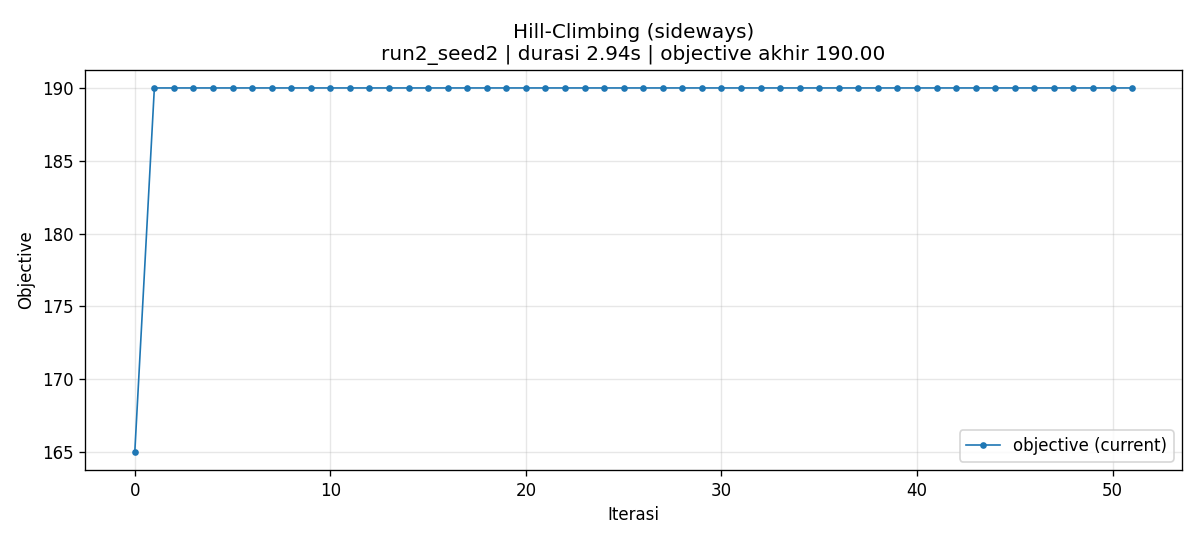
\includegraphics[width=0.48\textwidth]{hc/test_case/sideways/run2_seed2/objective.png}\hfill
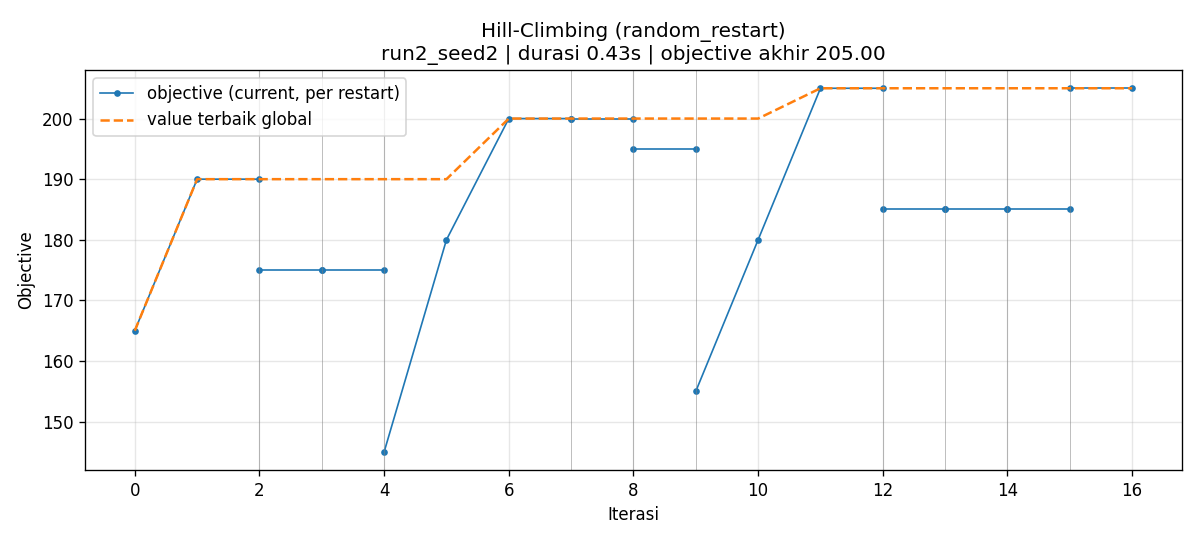
\includegraphics[width=0.48\textwidth]{hc/test_case/random_restart/run2_seed2/objective.png}
\caption{Objective terhadap iterasi seed 2: Sideways Move (kiri) dan Random Restart (kanan)}
\end{figure}

Pada seed 2, Steepest Ascent, Sideways Move, dan Stochastic sama-sama tertahan di local optimum
bernilai 190. Sideways Move menghabiskan 50 langkah datar tanpa menemukan jalan naik, sedangkan
Random Restart menemukan 205 pada restart ke-6.

\subsection{Simulated Annealing}
\begin{table}[H]
\centering
\caption{Hasil Simulated Annealing pada test\_case}\label{tab:hasilsa}
\small
\begin{tabular}{|C{1.2cm}|C{1.6cm}|C{1.8cm}|C{1.8cm}|C{1.5cm}|C{2.6cm}|C{1.6cm}|}
\hline
\hd{Seed} & \hd{Value awal} & \hd{Value state akhir} & \hd{best\_valid} & \hd{Iterasi} & \hd{Stuck (per 1.000 iter)} & \hd{Durasi (s)} \\ \hline
1 & 205 & 200 & 205 & 9.206 & 18 (1,96) & 2,76 \\ \hline
2 & 165 & 205 & 205 & 9.206 & 17 (1,85) & 3,60 \\ \hline
3 & 135 & 205 & 205 & 9.206 & 16 (1,74) & 3,65 \\ \hline
\end{tabular}
\end{table}

Dari 9.206 iterasi, langkah yang menurunkan objective dan tetap diterima berjumlah 124 (seed 1),
119 (seed 2), dan 108 (seed 3). Sebagian besar langkah diterima lainnya adalah langkah datar
($\Delta E = 0$, peluang 1).

\begin{figure}[H]
\centering
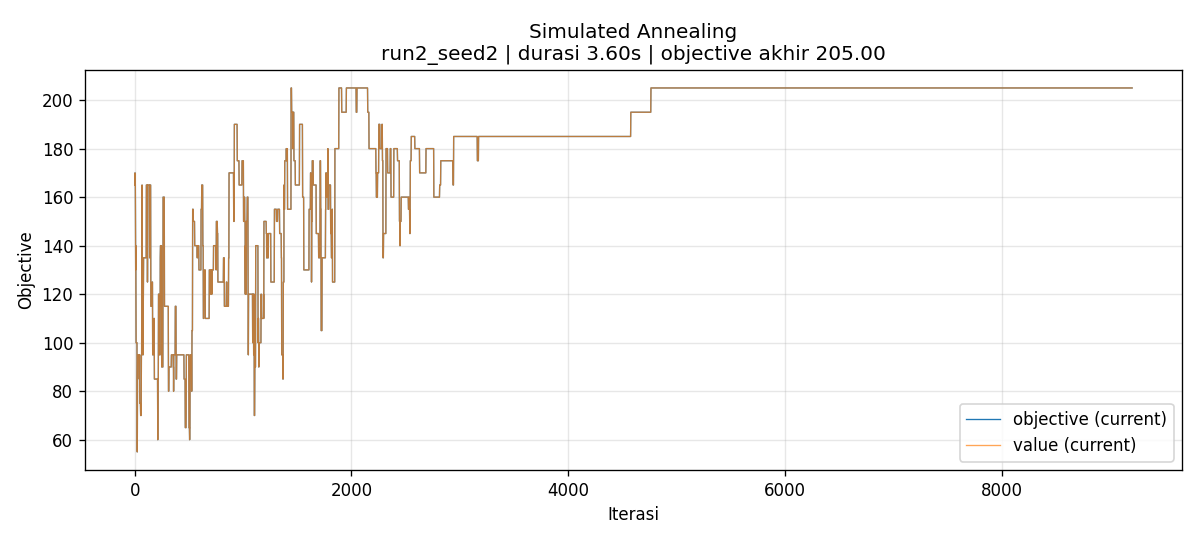
\includegraphics[width=0.48\textwidth]{sa/test_case/default/run2_seed2/objective.png}\hfill
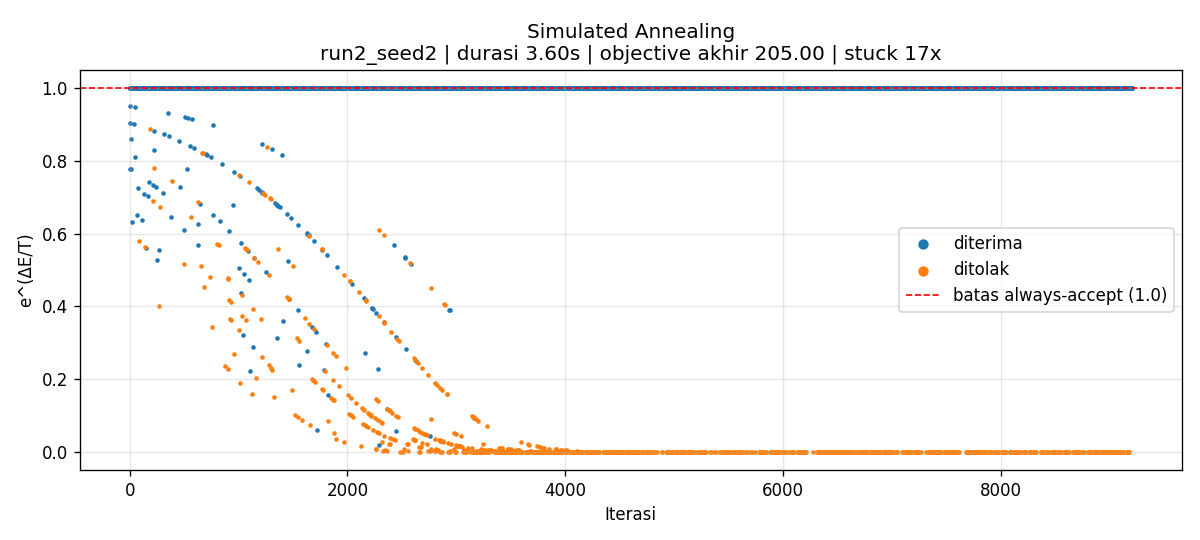
\includegraphics[width=0.48\textwidth]{sa/test_case/default/run2_seed2/accept_prob.png}
\caption{SA seed 2: objective terhadap iterasi (kiri) dan $e^{\Delta E/T}$ terhadap iterasi (kanan)}
\end{figure}

\begin{figure}[H]
\centering
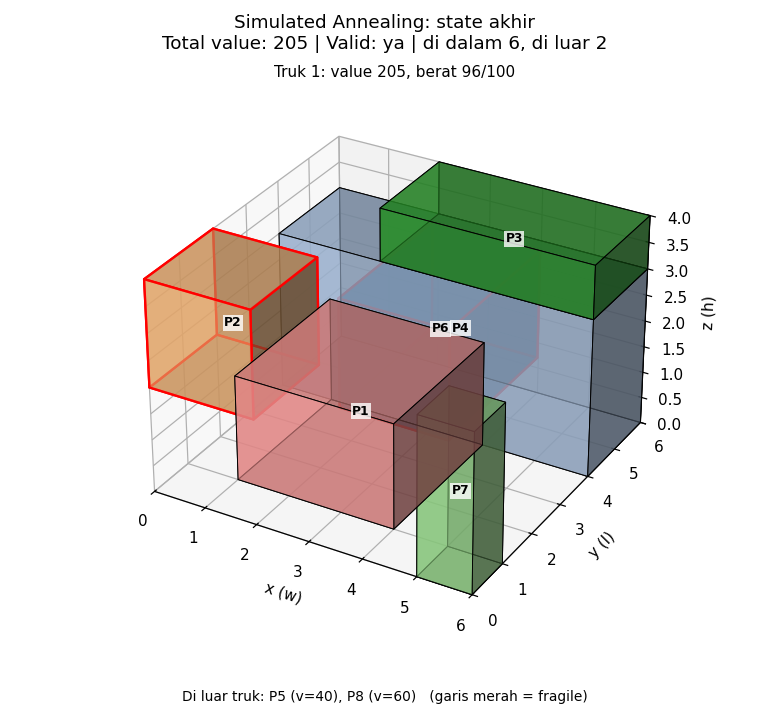
\includegraphics[width=0.6\textwidth]{sa/test_case/default/run2_seed2/final_state.png}
\caption{State akhir Simulated Annealing seed 2 (value 205)}
\end{figure}

\subsection{Genetic Algorithm}
\begin{table}[H]
\centering
\caption{Hasil Genetic Algorithm pada test\_case}\label{tab:hasilga}
\small
\begin{tabular}{|C{1.6cm}|C{1.6cm}|C{1.4cm}|C{2.8cm}|C{3.2cm}|C{1.8cm}|}
\hline
\hd{Eksp.} & \hd{Populasi} & \hd{Iterasi} & \hd{best\_valid (seed 1/2/3)} & \hd{Durasi (s, seed 1/2/3)} & \hd{Rata-rata (s)} \\ \hline
A & 50 & 50  & 205 / 205 / 205 & 1,52 / 1,75 / 1,79 & 1,69 \\ \hline
A & 50 & 100 & 205 / 205 / 205 & 2,05 / 2,46 / 2,29 & 2,27 \\ \hline
A & 50 & 200 & 205 / 205 / 205 & 3,38 / 4,10 / 3,91 & 3,80 \\ \hline
B & 20 & 100 & 205 / 205 / 205 & 1,10 / 1,09 / 1,04 & 1,08 \\ \hline
B & 50 & 100 & 205 / 205 / 205 & 2,06 / 2,57 / 2,25 & 2,29 \\ \hline
B & 100 & 100 & 205 / 205 / 205 & 4,29 / 4,15 / 4,74 & 4,39 \\ \hline
\end{tabular}
\end{table}

\begin{figure}[H]
\centering
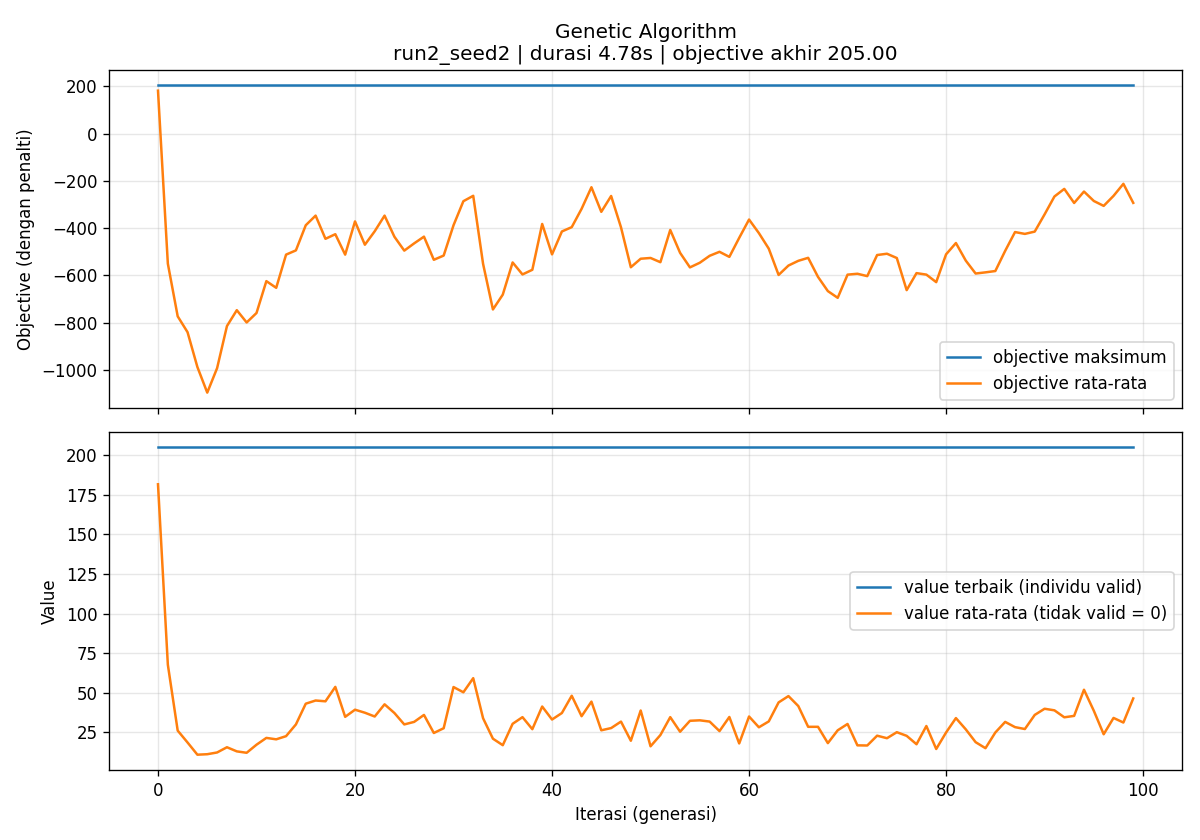
\includegraphics[width=0.75\textwidth]{ga/test_case/eksperimen_B/pop50_iter100/run2_seed2/objective.png}
\caption{Objective maksimum dan rata-rata populasi GA (populasi 50, iterasi 100, seed 2)}
\end{figure}

\begin{figure}[H]
\centering
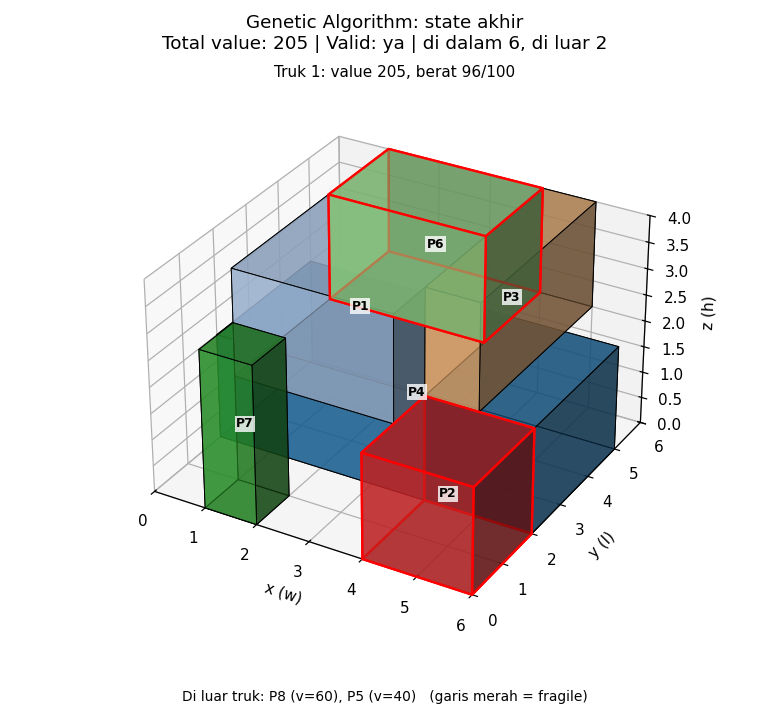
\includegraphics[width=0.6\textwidth]{ga/test_case/eksperimen_B/pop50_iter100/run2_seed2/final_state.png}
\caption{Individu terbaik GA (populasi 50, iterasi 100, seed 2; value 205)}
\end{figure}

\section{Analisis Hasil}
\subsection{Kedekatan dengan Optimum Global}
\begin{itemize}[leftmargin=1.5cm]
  \item GA mencapai optimum 205 di seluruh 18 run, dan SA di ketiga run (dilihat dari \code{best\_valid}).
  \item HC Random Restart mencapai 205 pada 2 dari 3 run; seed 3 berhenti di 200.
  \item Steepest Ascent, Sideways Move, dan Stochastic hanya mencapai optimum pada seed 1, yang memang sudah dimulai dari state optimum.
\end{itemize}
Penerimaan langkah turun memungkinkan SA keluar dari local optimum 190 dan 150 yang menahan
HC. Pada seed 3, SA naik dari 135 ke 205, sedangkan Steepest Ascent dari state yang sama berhenti
di 150.

\subsection{Perbandingan Hasil Antaralgoritma}
Urutan kualitas hasil pada test\_case adalah GA $\approx$ SA $>$ HC Random Restart $>$ HC Sideways
$>$ HC Steepest $=$ HC Stochastic. Sideways Move sedikit lebih baik pada seed 3 (185 dibanding 150)
karena langkah datar membawanya ke daerah dengan jalan naik. Stochastic memberi hasil
yang sama dengan Steepest Ascent di ketiga seed: keduanya mengevaluasi seluruh neighborhood dan
berhenti di local optimum yang sama, hanya jalur kenaikannya yang dapat berbeda.

\subsection{Perbandingan Durasi}
HC Steepest Ascent dan Stochastic paling cepat (sekitar 0,05 detik) karena hanya butuh 1--3
iterasi. Sideways Move paling lambat di antara varian HC (sekitar 2 detik) karena setiap langkah
datar tetap mengenumerasi seluruh neighbor. SA selalu menjalankan 9.206 iterasi dengan durasi 3--4
detik. Durasi GA tumbuh hampir linear terhadap populasi dan iterasi.

\subsection{Konsistensi Hasil}
GA dan SA paling konsisten (\code{best\_valid} 205 di semua seed). HC Steepest dan Stochastic
paling bergantung pada initial state (205 / 190 / 150). Random Restart mengurangi ketergantungan
tersebut dengan mengambil hasil terbaik dari 11 titik awal.

\subsection{Pengaruh Populasi dan Iterasi pada GA}
Variasi populasi dan iterasi tidak mengubah kualitas hasil pada test\_case karena individu terbaik
generasi 0 sudah bernilai 205: dengan hanya delapan paket, populasi acak sudah memuat optimum.
Rata-rata objective populasi turun tajam setelah generasi 0 (dari 181,6 menjadi $-600{,}9$ pada generasi 1) karena
crossover uniform sering menghasilkan anak tidak valid yang terkena penalti $\lambda$; jumlah
individu valid turun dari 50 menjadi 20. Untuk dataset sekecil ini, populasi 20
dengan 100 iterasi sudah cukup.

\subsection{Perilaku Simulated Annealing}
Dengan penerimaan probabilistik, plot $e^{\Delta E/T}$ menunjukkan nilai yang tinggi di awal
(langkah buruk sering diterima) dan mendekati nol setelah suhu turun, kecuali $\Delta E = 0$ yang
selalu bernilai 1. Pada seed 1, SA sempat meninggalkan state optimum 205 dan berakhir di 200,
sehingga penyimpanan \code{best\_valid} tetap penting. Frekuensi stuck sekitar 1,7--2 kejadian per
1.000 iterasi; angka ini juga menghitung jendela setelah optimum ditemukan, sehingga lebih tepat
dibaca sebagai banyaknya jendela 500 iterasi tanpa perbaikan.

% =====================================================================
\chapter{KESIMPULAN \& SARAN}
% =====================================================================

\section{Kesimpulan}
\begin{enumerate}[leftmargin=1.5cm]
  \item Persoalan pengisian peti kemas Mejiro Express berhasil diselesaikan dengan empat varian Hill-Climbing, Simulated Annealing, dan Genetic Algorithm yang berbagi representasi state, pengecekan constraint, dan operator neighbor yang sama.
  \item Pada test\_case, optimum global 205 dicapai oleh seluruh 18 run GA, ketiga run SA, 2 dari 3 run HC Random Restart, dan 1 dari 3 run untuk varian HC lainnya.
  \item Algoritma yang mampu keluar dari local optimum (SA) atau mencoba banyak titik awal (GA dan Random Restart) secara konsisten lebih baik daripada HC biasa.
  \item Variasi populasi dan iterasi GA pada test\_case hanya memengaruhi durasi, bukan kualitas hasil.
  \item Bonus OF prioritas ETA, keempat varian HC, dan multi-truk berhasil diimplementasikan tanpa perubahan pada kode algoritma inti.
\end{enumerate}

\section{Keterbatasan}
\begin{enumerate}[leftmargin=1.5cm]
  \item Pengujian hanya dilakukan pada test\_case yang berukuran kecil, sehingga perbedaan antaralgoritma, terutama pengaruh parameter GA, belum terlihat penuh.
  \item Seluruh varian HC mengenumerasi seluruh neighbor, sehingga biaya per iterasinya tumbuh cepat pada truk besar dengan banyak paket.
  \item Definisi melayang mengikuti spesifikasi secara harfiah (cukup satu titik alas ditopang), sehingga paket boleh menggantung sebagian.
\end{enumerate}

\section{Saran}
\begin{enumerate}[leftmargin=1.5cm]
  \item Menguji ulang pada dataset yang lebih besar agar pengaruh populasi dan iterasi GA terlihat.
  \item Membatasi neighborhood HC, misalnya hanya mencoba posisi yang menempel pada dinding atau paket lain.
  \item Mengubah definisi stuck SA agar hanya dihitung sebelum solusi terbaik ditemukan.
\end{enumerate}

% =====================================================================
\begin{thebibliography}{9}
\addcontentsline{toc}{chapter}{DAFTAR PUSTAKA}
\bibitem{khodra1} M. L. Khodra, ``Beyond Classical Search: Classical vs Local Search,'' YouTube, 2021. [Video].
\bibitem{khodra2} M. L. Khodra, ``Beyond Classical Search: State (Value, Neighbor),'' YouTube, 2021. [Video]. Available: \url{https://www.youtube.com/watch?v=_6rla37QorM}
\bibitem{khodra3} M. L. Khodra, ``Beyond Classical Search: Hill-climbing Search,'' YouTube, 2021. [Video]. Available: \url{https://www.youtube.com/watch?v=L0b0CN3Fds8}
\bibitem{khodra4} M. L. Khodra, ``Beyond Classical Search: Simulated Annealing,'' YouTube, 2021. [Video].
\bibitem{khodra5} M. L. Khodra, ``Beyond Classical Search: Genetic Algorithm,'' YouTube, 2021. [Video].
\bibitem{aima} S. Russell dan P. Norvig, \textit{Artificial Intelligence: A Modern Approach}, 4th ed. Hoboken, NJ: Pearson, 2020.
\end{thebibliography}

% =====================================================================
\section*{Lampiran A. Pembagian Tugas}
\phantomsection\addcontentsline{toc}{section}{Lampiran A. Pembagian Tugas}
\begin{table}[H]
\centering
\small
\begin{tabular}{|L{2.4cm}|L{4.6cm}|L{6.2cm}|}
\hline
\hd{NIM} & \hd{Nama} & \hd{Tugas} \\ \hline
13524028 & Muhammad Nur Majiid & Model data dan Genetic Algorithm \\ \hline
13524064 & Stefani Angeline Oroh & Algoritma Hill-Climbing dan laporan \\ \hline
13524079 & Angelina Andra Alanna & Fungsi objektif, Simulated Annealing, visualisasi, dan laporan \\ \hline
\end{tabular}
\end{table}

\section*{Lampiran B. Form Penggunaan Generative AI}
\phantomsection\addcontentsline{toc}{section}{Lampiran B. Form Penggunaan Generative AI}
\begin{center}
{\bfseries FORMAT DEKLARASI PENGGUNAAN AI\\ SURAT PERNYATAAN PENGGUNAAN AI\par}
\end{center}
\noindent Dengan ini, kami:\par
\begin{tabular}{@{\hspace{0.5cm}}l@{\hspace{0.4cm}}l@{\hspace{0.3cm}}L{8.8cm}}
Nama/NIM & : & Muhammad Nur Majiid / 13524028 \\
         &   & Stefani Angeline Oroh / 13524064 \\
         &   & Angelina Andra Alanna / 13524079 \\
Fakultas/Sekolah & : & Sekolah Teknik Elektro dan Informatika (STEI) \\
Kode Mata Kuliah & : & IF3170 \\
Nama Mata Kuliah & : & Inteligensi Artifisial \\
Judul Tugas/Proposal & : & Tugas Besar 1: Local Search untuk Optimasi Pengisian Peti Kemas Truk \\
\end{tabular}

\medskip
\noindent menyatakan bahwa kami \textbf{menggunakan} AI dalam pengerjaan maupun penyusunan luaran
tugas pada mata kuliah yang tertulis di atas. Alat AI/kecerdasan buatan yang digunakan adalah:

\begin{table}[H]
\centering
\small
\begin{tabular}{|L{6.4cm}|C{2.2cm}|L{4.6cm}|}
\hline
\hd{Lingkup Pekerjaan} & \hd{Digunakan?} & \hd{Tingkat Penggunaan} \\ \hline
\textbf{Pemeriksaan Ejaan:} menggunakan tools seperti Grammarly, Paperpal, DeepL, Quillbot,
Grammarbot, LanguageTool, ProWritingAid, ChatGPT, Google Gemini, atau sejenisnya.
 & Ya & Memeriksa ejaan dan tata bahasa teks laporan \\ \hline
\textbf{Pembuatan Teks:} menggunakan tools seperti ChatGPT, Gemini, Paperpal, Copilot,
GrammarlyGO, WordAI, WriteSonic, Jasper, Jenni AI, atau sejenisnya.
 & Tidak & -- \\ \hline
\textbf{Bantuan Diskusi dalam Penyusunan Konten:} menggunakan tools seperti ChatGPT, Gemini,
Copilot, Perplexity, Jenni AI, Zoom-Companion, atau sejenisnya.
 & Ya & Membantu memahami salindia perkuliahan \\ \hline
\textbf{Pembuatan Gambar, Video, dan/atau Grafik:} menggunakan tools seperti Craiyon, DALL-E,
Midjourney, Stable Diffusion, Microsoft Designer, Gemini, Canva AI, atau sejenisnya.
 & Ya & Google Gemini untuk membuat ilustrasi constraint dan orientasi paket
       (Gambar~\ref{fig:constraint} dan \ref{fig:orientasi}) agar penjelasan tertulis lebih mudah divisualisasikan \\ \hline
\textbf{Lainnya, Jelaskan:} & -- & -- \\ \hline
\end{tabular}
\end{table}

\noindent Kami juga menyatakan bahwa setiap penggunaan AI/kecerdasan buatan yang dilakukan pada
mata kuliah tersebut telah dinyatakan di dalam surat ini.

\vspace{0.8cm}
\noindent\hfill Bandung, 20 Oktober 2026\par
\vspace{0.4cm}
\noindent
\begin{tabular}{C{4.3cm}C{4.3cm}C{4.3cm}}
\parbox[b][1.6cm][b]{3.6cm}{\centering
\includegraphics[height=1.5cm,width=3.6cm,keepaspectratio]{ttd_majid_crop.png}} &
\parbox[b][1.6cm][b]{3.6cm}{\centering
\includegraphics[height=1.5cm,width=3.6cm,keepaspectratio]{ttd_angel_crop.png}} &
\parbox[b][1.6cm][b]{3.6cm}{\centering
\includegraphics[height=1.5cm]{ttd_andra_crop.png}} \\
\rule{3.6cm}{0.4pt} & \rule{3.6cm}{0.4pt} & \rule{3.6cm}{0.4pt} \\
Muhammad Nur Majiid & Stefani Angeline Oroh & Angelina Andra Alanna \\
13524028 & 13524064 & 13524079 \\
\end{tabular}

\section*{Lampiran C. Tautan Repository}
\phantomsection\addcontentsline{toc}{section}{Lampiran C. Tautan Repository}
\url{https://github.com/MAJIIDMN/IF3170_G15_WedaBest}

\end{document}
